% ══════════════════════════════════════════════════════════════════
\chapter{Geometry Revisited: The PCA Metric Was Wrong}
\label{ch:geometry}
% ══════════════════════════════════════════════════════════════════

\noindent
\textbf{Experimental setup.}
Fashion-MNIST (2000 samples), depths $L \in \{5, 10, 15, 20\}$,
width~784 (square projections).  Five initializers compared using the
three geometry metrics from Section~\ref{sec:geometry_metrics}.

% ──────────────────────────────────────────────────────────────────
\section{$k$-NN Results Overturn the Narrative}

\begin{table}[h]
\centering
\begin{tabular}{lcccc}
\toprule
Initializer & 5\,L & 10\,L & 15\,L & 20\,L \\
\midrule
\texttt{he}                          & 0.736 & 0.710 & 0.673 & \textbf{0.639} \\
\texttt{orthogonal\_he}              & \textbf{0.755} & \textbf{0.724} & \textbf{0.696} & \textbf{0.662} \\
\texttt{orthogonal\_tuned}           & 0.755 & 0.724 & 0.696 & 0.662 \\
\texttt{row\_centered\_he\_var\_adj} & 0.717 & 0.482 & 0.186 & 0.110 \\
\texttt{kernel\_preserving}          & 0.737 & 0.628 & 0.540 & 0.100 \\
\bottomrule
\end{tabular}
\caption{$k$-NN accuracy ($k=5$) vs.\ depth.
  Chance level $= 0.10$ (10 classes).}
\label{tab:knn}
\end{table}

\textbf{The key finding:}
Row-centered var-adj drops from 0.717 (5\,L) to \textbf{0.110} (20\,L)
--- indistinguishable from \textbf{chance level}.
Meanwhile He degrades gracefully from 0.736 to 0.639, losing only
$\sim$13\% of its class separability over 20 layers.

This directly contradicts the PCA scatter plot evidence from earlier
work, which suggested row centering ``preserves geometry'' better
than~He.

\begin{figure}[h]
\centering
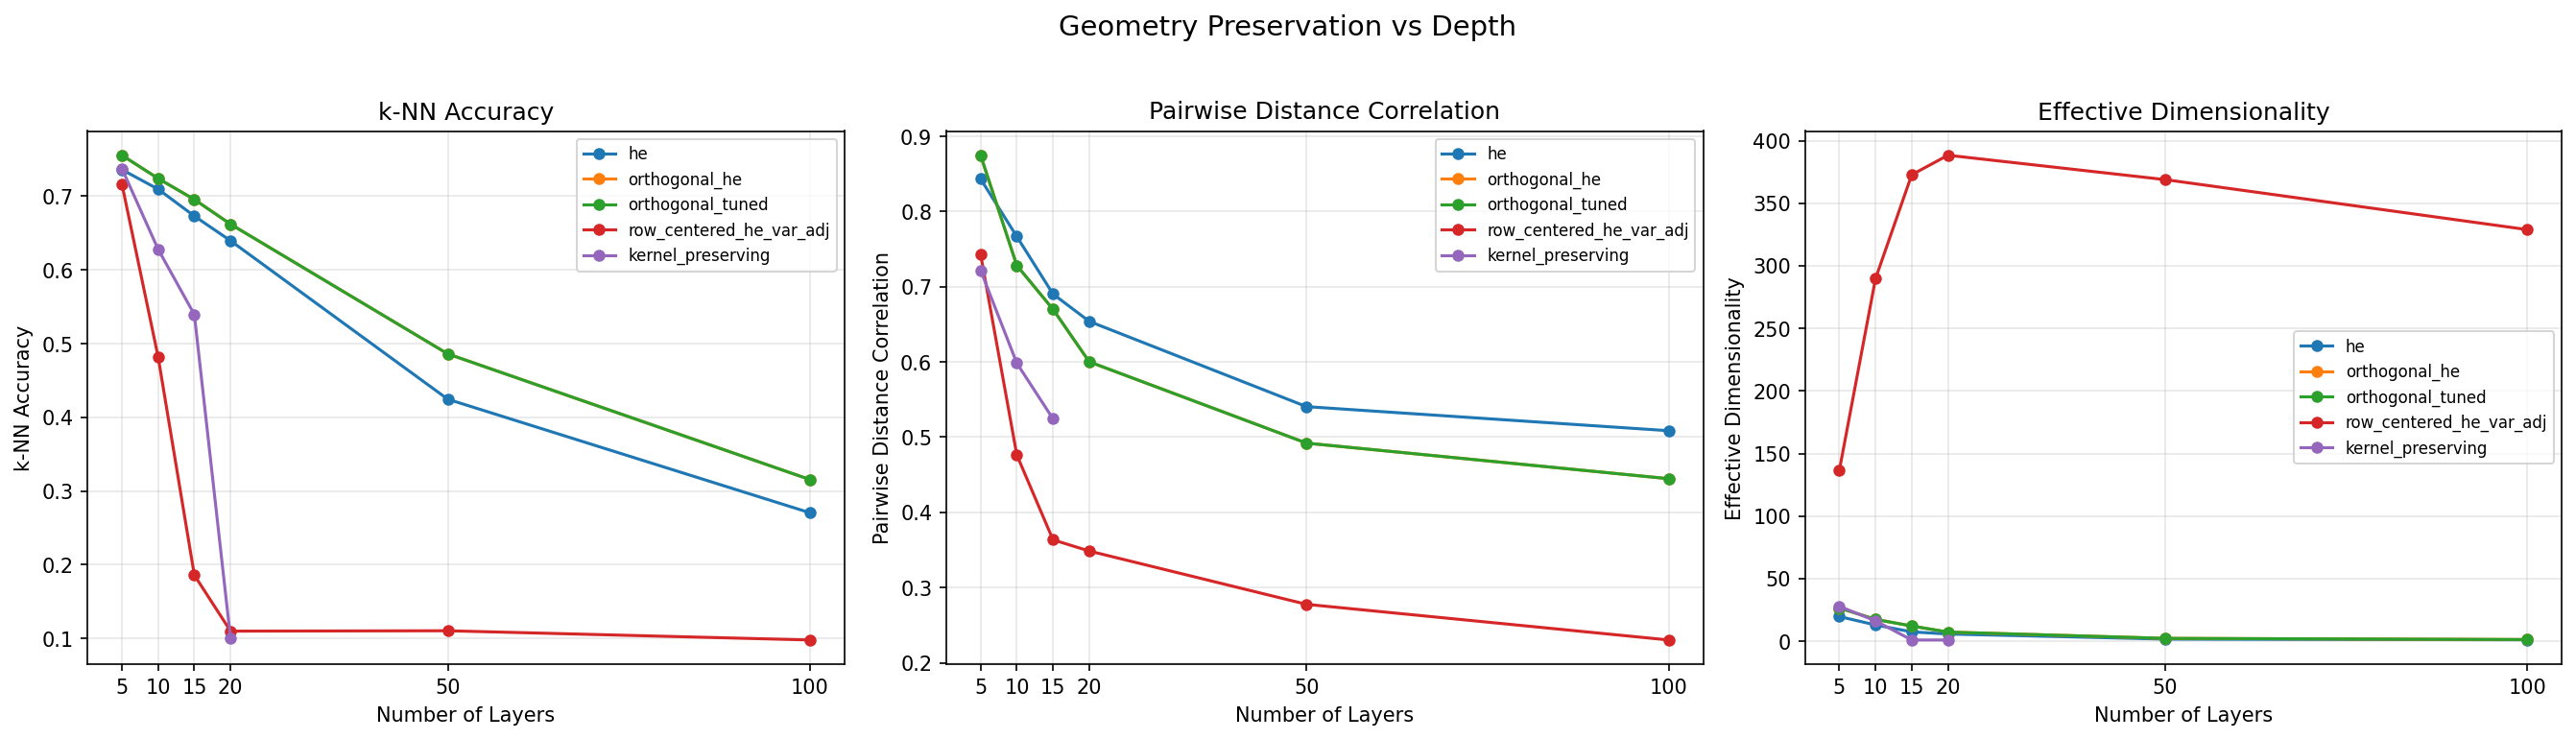
\includegraphics[width=\textwidth]{figures/geometry_vs_depth.png}
\caption{Three geometry metrics vs.\ depth for five initializers.
  \textbf{Left:} $k$-NN accuracy --- row-centered drops to chance (0.10)
  by 20~layers while He stays at 0.64.
  \textbf{Center:} Pairwise distance correlation.
  \textbf{Right:} Effective dimensionality --- row-centered has high
  $d_{\mathrm{eff}}$ (spread-out noise) despite zero class structure.
  Source: \texttt{notebooks/07\_kernel\_geometry\_analysis.ipynb}, Cell~6.}
\label{fig:geometry_vs_depth}
\end{figure}

\begin{table}[h]
\centering
\begin{tabular}{lcccc}
\toprule
Initializer & 5\,L & 10\,L & 15\,L & 20\,L \\
\midrule
\texttt{he}                          & 0.843 & 0.767 & 0.690 & 0.654 \\
\texttt{orthogonal\_he}              & \textbf{0.875} & 0.728 & 0.670 & 0.600 \\
\texttt{row\_centered\_he\_var\_adj} & 0.743 & 0.476 & 0.363 & 0.349 \\
\texttt{kernel\_preserving}          & 0.722 & 0.598 & 0.524 & NaN \\
\bottomrule
\end{tabular}
\caption{Pairwise distance correlation (Spearman) vs.\ depth.}
\label{tab:dist_corr}
\end{table}

\begin{table}[h]
\centering
\begin{tabular}{lcccc}
\toprule
Initializer & 5\,L & 10\,L & 15\,L & 20\,L \\
\midrule
\texttt{he}                          & 19.7 & 13.0 & 7.5 & 5.8 \\
\texttt{orthogonal\_he}              & 26.6 & 17.5 & 12.2 & 7.3 \\
\texttt{row\_centered\_he\_var\_adj} & \textbf{136.2} & \textbf{289.7} & \textbf{372.7} & \textbf{388.3} \\
\texttt{kernel\_preserving}          & 28.0 & 16.3 & 1.0 & 1.0 \\
\bottomrule
\end{tabular}
\caption{Effective dimensionality (eigenvalue entropy) vs.\ depth.}
\label{tab:eff_dim}
\end{table}

% ──────────────────────────────────────────────────────────────────
\section{Why the PCA Metric Was Misleading}
\label{sec:pca_misleading}

The effective dimensionality reveals the mechanism:
\begin{itemize}
  \item \textbf{Row-centered}: $d_{\mathrm{eff}} = 388$ at 20\,L
        (data spread across $\sim$388 dimensions).
  \item \textbf{He}: $d_{\mathrm{eff}} = 5.8$ at 20\,L
        (data compressed into $\sim$6 dimensions).
\end{itemize}

The PCA scatter plots showed row-centered data ``spreading out'' in the
first two principal components --- which \emph{looks like} preserved
structure.  But \textbf{spread $\neq$ structure}:

\begin{enumerate}
  \item The forward signal decays by $0.826^L$ per layer
        (equation~\eqref{eq:compounding}).
  \item By 20 layers: $0.826^{20} \approx 0.022$, so activations are
        $\sim\!46\times$ smaller than the input.
  \item At this scale, the signal is dominated by random fluctuations
        from weight initialization, not input structure.
  \item The data becomes \textbf{uniformly dispersed noise}: high
        dimensional (high $d_{\mathrm{eff}}$) but with
        \emph{no class information} ($k$-NN $=$ chance).
\end{enumerate}

He, by contrast, compresses data into fewer dimensions (low
$d_{\mathrm{eff}}$), but the \textbf{class structure is preserved
within those dimensions}.  The angular contraction from the ReLU kernel
($D(\alpha) > 0$) compresses representations but maintains relative
ordering of inter-class vs.\ intra-class distances.

\begin{remark}[Effective dimensionality is misleading in isolation]
High $d_{\mathrm{eff}}$ combined with low $k$-NN accuracy indicates
uniformly dispersed noise, not good geometry.
Low $d_{\mathrm{eff}}$ combined with high $k$-NN accuracy indicates
efficient compression with preserved class structure.
The $k$-NN accuracy is the correct primary metric.
\end{remark}

% ──────────────────────────────────────────────────────────────────
\section{Orthogonal Initialization Analysis}
\label{sec:orthogonal_analysis}

\subsection{Same expected kernel as He}

\begin{proposition}
For a square orthogonal matrix $W = \sqrt{2}\,Q$ (where $Q$ is from QR
decomposition), the expected kernel per neuron is the same as for
i.i.d.\ Gaussian weights with matching variance.
\end{proposition}

\begin{proof}[Proof sketch]
Each row $\bm{w}_k$ of the orthogonal matrix, viewed in isolation,
is uniformly distributed on the sphere of radius $\sqrt{2}$.
This is the same distribution as a normalized Gaussian vector
$\sqrt{2}\,\bm{g}/\|\bm{g}\|$ where $\bm{g} \sim \mathcal{N}(\bm{0}, I)$.
In the large-$d$ limit, $\|\bm{g}\| \approx \sqrt{d}$ concentrates, so
the marginal distribution of $\bm{w}_k$ approaches
$\mathcal{N}(\bm{0}, (2/d)\,I)$ --- the same as He.

The kernel proof (Theorem~\ref{thm:kernel}) computes
$\E[\relu(\bm{w}_k^\top \bm{x}_i) \cdot \relu(\bm{w}_k^\top \bm{x}_j)]$,
which depends only on the marginal distribution of individual rows.
Since orthogonal rows have the same marginal as Gaussian rows, the
expected kernel per neuron is identical.
\end{proof}

\textbf{What orthogonal changes:} The rows are no longer independent
(they are mutually orthogonal), so the \emph{variance} of the kernel
estimate decreases (better concentration).  The \emph{expectation} is
still $K(\alpha)$ with the same distortion $D(\alpha) > 0$.

\textbf{Prediction confirmed:} Orthogonal shows the same systematic
collapse rate as He, with ${\sim}3.6\%$ improvement from reduced noise
($0.662$ vs.\ $0.639$ at 20\,L).

\subsection{Orthogonal\_he equals orthogonal\_tuned}

With square matrices ($784 \times 784$) and the same seed, QR produces
the same orthogonal matrix $Q$.  The only difference is the gain:
$\sqrt{2}\,Q$ vs.\ $\sqrt{1.65}\,Q$.  Since all three geometry metrics
($k$-NN, Spearman distance correlation, effective dimensionality) are
\textbf{scale-invariant}, the two produce identical results.

% ──────────────────────────────────────────────────────────────────
\section{Kernel-Preserving Failure at Depth}
\label{sec:kp_failure}

\begin{center}
\begin{tabular}{ccccc}
\toprule
Depth & $k$-NN & Dist.\ corr. & $d_{\mathrm{eff}}$ & Status \\
\midrule
5\,L  & 0.737 & 0.722 & 28.0 & Comparable to He \\
10\,L & 0.628 & 0.598 & 16.3 & Degrading \\
15\,L & 0.540 & 0.524 & 1.0  & Numerical collapse \\
20\,L & 0.100 & NaN   & 1.0  & Overflow \\
\bottomrule
\end{tabular}
\end{center}

The kernel-preserving optimizer (Section~\ref{sec:kp_init}) optimizes
each layer independently via 200~Adam steps.  It does not account for
how previous layers have already transformed the data.

\begin{itemize}
  \item At 5\,L: comparable to He ($0.737$ vs.\ $0.736$).
  \item At 15\,L: $d_{\mathrm{eff}} = 1.0$ --- data has collapsed to a
        single direction.
  \item At 20\,L: $k$-NN $= 0.100$ (chance), distance correlation $=$ NaN
        (float64 overflow from accumulated weight inflation of
        ${\sim}15^{20}$).
\end{itemize}

Per-layer optimization is \textbf{non-composable}: each layer is
locally optimal, but the composition of 15+ independently-optimized
layers diverges.

% ──────────────────────────────────────────────────────────────────
\section{Revised Narrative}
\label{sec:revised_narrative}

The previous argument was:
\begin{quote}
\emph{``Row centering preserves geometry but creates a gradient trap.''}
\end{quote}

The corrected argument is:
\begin{quote}
\textbf{Row centering prevents angular collapse but destroys class
structure (via forward signal decay) AND creates a gradient trap.
These are the same phenomenon --- the forward decay kills both.}
\end{quote}

Row centering:
\begin{enumerate}
  \item Does \textbf{NOT} preserve geometry (as measured by class
        separability / $k$-NN accuracy).
  \item \textbf{DOES} prevent angular collapse (data stays spread out
        --- high $d_{\mathrm{eff}}$).
  \item But ``staying spread out'' $\neq$ ``preserving structure.''
        The data gets randomized into high-dimensional noise.
\end{enumerate}
